\clearpage
\subsection{premi/client/frameEditor}
\begin{figure}[h]
\begin{center}
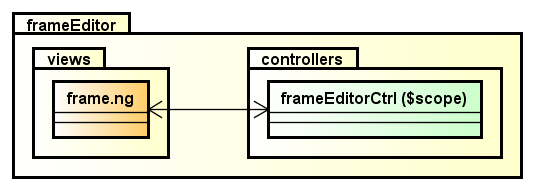
\includegraphics[scale=0.55]{img/diapkg/frameEditor.png}
\caption{Diagramma del package premi/client/frameEditor}
\end{center}
\end{figure}

%-------  diagramma di un template %
\subsubsection{premi/client/frameEditor/views/frame.ng}

\begin{description}
%-------  descrizione del template%
\item[Descrizione] \hfill
	Template della vista associata allo \textit{\$scope} di \textit{frameEditorCtrl}. Fornisce tutti gli strumenti necessari alla creazione di un frame, tra cui:
	\begin{itemize}
			\item creazione, modifica e rimozione di frame
			\item inserimento, modifica e rimozione di immagini, shape, e testo
			\item spostamento di immagini, shape  e testo all'interno del frame
	\end{itemize}
\end{description}








%-------  diagramma della classe%
\subsubsection{premi/client/frameEditor/controllers/frameEditorCtrl}
\begin{figure}[h]
\begin{center}
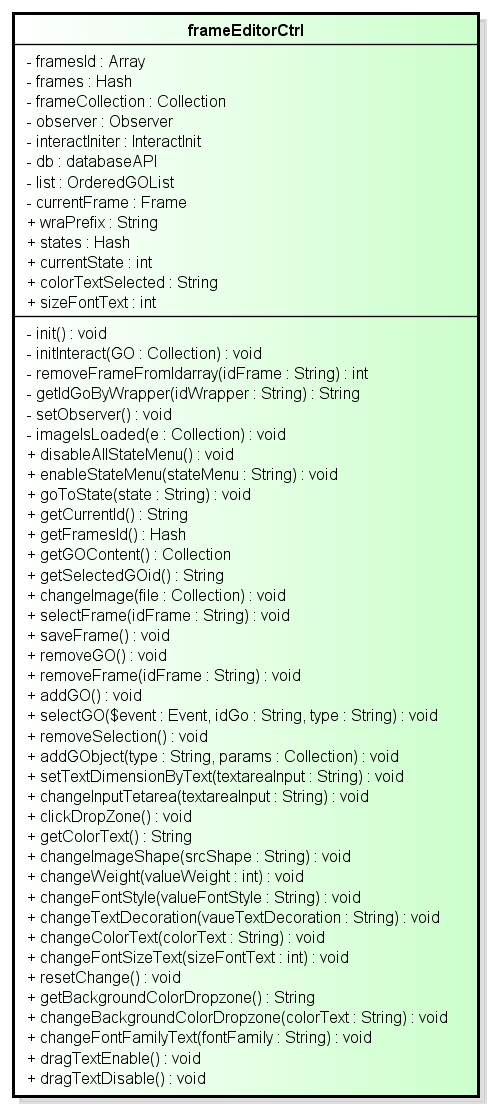
\includegraphics[scale=0.47]{img/diacla/frameEditorCtrl.png}
\caption{Diagramma della classe premi/client/frameEditor/controllers/frameEditorCtrl}
\end{center}
\end{figure}


\begin{description}
%-------  descrizione della classe%
\item[Descrizione] \hfill
	Questo controller crea lo \$scope associato alla vista generata da \textbf{frame.ng}, fornendo i dati e i metodi necessari per consentire all'utente di creare e modellare un frame, inserendo o rimuovendo oggetti grafici al suo interno.
	
	
%-------  lista delle classi associate%	
\item[Dipendenze] \hfill
	\begin{itemize}
		\item \textbf{premi/client/presentation/lib/OrderedGoList}: per la gestione degli oggetti grafici contenuti nei frame
		\item \textbf{premi/client/presentation/lib/databaseAPI}: per il salvataggio dei frame nel database
		\item \textbf{premi/client/editor/lib/InteractInit}: per accedere alla libreria Interact.JS e offrire una rappresentazione grafica dei frame all'utente
		\item \textbf{premi/client/editor/lib/Frame}: per la creazione e la modifica dei frame
		\item \textbf{premi/client/editor/lib/Observer}: per dare un Observer agli oggetti che ne fanno uso
	\end{itemize}
	
	
%-------  lista degli Attributi%	
\item[Attributi] \hfill
	\begin{description}
		\item[\textbf{- framesId : Array			}] \hfill
			Array dei codici identificativi dei frame creati dall'utente nella presentazione che sta modificando
		\item[\textbf{- frames : Hash			}] \hfill
			Hash dei frames creati dall'utente in questa presentazione, strutturato come \textit{id\_frame} : \textit{Collezione JSON dei suoi attributi}
		\item[\textbf{- frameCollection : Collection			}] \hfill
			Collezione di MongoDB dei frames contenuti nella presentazione che l'utente sta modificando
		\item[\textbf{- observer : Observer			}] \hfill
			Observer della classe, che andrà associato agli oggetti con cui l'utente lavora
		\item[\textbf{- interactIniter : InteractInit			}] \hfill
			interactIniter è utilizzato per l'inizializzazione della libreria Interact.JS
		\item[\textbf{- db : databaseAPI			}] \hfill
			Contiene una lista di metodi coi quali la classe può salvare i dati dell'utente nel database
		\item[\textbf{- list : OrderedGOList			}] \hfill
			È la lista di oggetti grafici contenuti nel frame che l'utente sta modificando
		\item[\textbf{- currentFrame : Frame			}] \hfill
			È il frame che l'utente sta modificando
		\item[\textbf{+ wraPrefix : String			}] \hfill
			Stringa che indica quale prefisso si sta utilizzando per gli oggetti "wrapper" che compongono l'interfaccia grafica di questa parte di editor
		\item[\textbf{+ states : Hash			}] \hfill
			Oggetto contenente una lista di stati che l'editor può assumere durante il suo utilizzo da parte dell'utente. Una volta inizializzato non può più essere modificato. Inizializzarlo con i seguenti campi:
		\begin{itemize}
			\item noSelection : 1
			\item imageEditing : 2
			\item shapeEditing : 3
			\item textEditing : 4
			\item addingGo : 5
			\item framesList : 6
		\end{itemize}
		\item[\textbf{+ currentState : int			}] \hfill
			Lo stato che l'editor sta assumendo. Il suo valore può essere solo uno tra quelli rappresentati da states
		\item[\textbf{+ currentImage : String			}] \hfill
			Il codice identificativo dell'immagine che l'utente sta utilizzando
		\item[\textbf{+ colorTextSelected : String			}] \hfill
			Il colore selezionato dall'utente nell'editor
		\item[\textbf{+ sizeFontText : int			}] \hfill
			La dimensione del testo selezionata dall'utente nell'editor
	\end{description}
	
	
%-------  lista dei metodi%	
\item[Metodi] \hfill

	% -- inizio metodo -- %
	\begin{description}
		\item[\textbf{\color{blue}- init() : void			}] \hfill
			Inizializza gli attributi della classe.
			
		\begin{description}
			
			% -- note aggiuntive sul metodo -- %
			\item[Note] \hfill
			\begin{itemize}
					\item chiama la classe setObserver()
					\item imposta l'Observer in interactIniter
					\item inizializza framesId e frames, prelevando le informazioni da framesCollection
					\item carica il primo frame, inizializzando list e currentFrame, e preparando la visualizzazione attraverso initInteract
			\end{itemize}
		\end{description}
	\end{description}
	% -- fine metodo -- %	
	
	
		% -- inizio metodo -- %
	\begin{description}
		\item[\textbf{\color{blue}- initInteract(GO : Collection) : void			}] \hfill
			Rappresenta in modo visivo all'utente l'oggetto grafico ricevuto, attraverso la libreria esterna Interact.JS. Utilizza i metodi initializeImage, initializeShape o initializeText di interactIniter, in base al tipo dell'oggetto grafico ricevuto.
			
		\begin{description}
			% -- lista argomenti del metodo -- %
			\item[Argomenti] \hfill
				\begin{itemize}
				
					\item \textbf{GO : Collection		} \hfill
					Collezione di attributi dell'oggetto grafico da rappresentare
					
				\end{itemize}
		\end{description}
	\end{description}
	% -- fine metodo -- %	
	
		% -- inizio metodo -- %
	\begin{description}
		\item[\textbf{\color{blue}- removeFrameFromIdarray(idFrame : String) : int			}] \hfill
			Rimuove il frame rappresentato dal codice identificativo ricevuto da framesId. Restituisce la posizione in cui si trovava il frame
			
		\begin{description}
			% -- lista argomenti del metodo -- %
			\item[Argomenti] \hfill
				\begin{itemize}
				
					\item \textbf{idFrame : String		} \hfill
					Il codice identificativo del frame da rimuovere
					
				\end{itemize}
				
		\end{description}
	\end{description}
	% -- fine metodo -- %				
	
	% -- inizio metodo -- %
	\begin{description}
		\item[\textbf{\color{blue}- getIdGoByWrapper() : String			}] \hfill
			Restituisce il codice identificativo dell'oggetto grafico estraendolo dal codice identificativo del wrapper (che sarà composto dall'unione tra wraPrefix e il codice identificativo dell'oggetto)
			
		\begin{description}
			% -- lista argomenti del metodo -- %
			\item[Argomenti] \hfill
				\begin{itemize}
				
					\item \textbf{idWrapper : String		} \hfill
					Il codice identificativo del wrapper
					
				\end{itemize}
				
		\end{description}
	\end{description}
	% -- fine metodo -- %	
	
	% -- inizio metodo -- %
	\begin{description}
		\item[\textbf{\color{blue}- setObserver() : void		}] \hfill
			Imposta l'observer per reagire agli eventi select, resize, drag, update e changeLvl inviati dalla vista, per l'aggiornamento degli attributi dell'oggetto grafico che sta venendo modificato dall'utente 
		
	\end{description}
	% -- fine metodo -- %		
	
	% -- inizio metodo -- %
	\begin{description}
		\item[\textbf{\color{blue}- imageIsLoaded(e : Collection) : void			}] \hfill
			Aggiorna il frame appena modificato con nuovi attributi
			
		\begin{description}
			% -- lista argomenti del metodo -- %
			\item[Argomenti] \hfill
				\begin{itemize}
				
					\item \textbf{e : Collection		} \hfill
					Collezione di attributi modificati dall'utente
					
				\end{itemize}
				
		\end{description}
	\end{description}
	% -- fine metodo -- %
	
	
	% -- inizio metodo -- %
	\begin{description}
		\item[\textbf{\color{blue}+ disableAllStateMenu() : void	}] \hfill
			Imposta currentState a states.noSelection 
		
	\end{description}
	% -- fine metodo -- %
	
	% -- inizio metodo -- %
	\begin{description}
		\item[\textbf{\color{blue}+ enableStateMenu(stateMenu : String) : void		}] \hfill
			Cambia currentState in base allo stato ricevuto
			
		\begin{description}
			% -- lista argomenti del metodo -- %
			\item[Argomenti] \hfill
				\begin{itemize}
				
					\item \textbf{stateMenu : String		} \hfill
					Lo stato in cui si trova l'editor
					
				\end{itemize}
				
		\end{description}
	\end{description}
	% -- fine metodo -- %
	
	% -- inizio metodo -- %
	\begin{description}
		\item[\textbf{\color{blue}+ goToState(state : String) : void  	}] \hfill
			Ridireziona il browser in base allo stato ricevuto
			
		\begin{description}
			% -- lista argomenti del metodo -- %
			\item[Argomenti] \hfill
				\begin{itemize}
				
					\item \textbf{state : String		} \hfill
					Il nuovo stato. In questo caso rappresenta una posizione, o pagina, all'interno dell'applicazione					
				\end{itemize}
				
		\end{description}
	\end{description}
	% -- fine metodo -- %
	
	
	% -- inizio metodo -- %
	\begin{description}
		\item[\textbf{\color{blue}+ getCurrentId() : String	}] \hfill
			Restituisce il codice identificativo del frame contenuto in currentFrame
		
	\end{description}
	% -- fine metodo -- %
	
	
	% -- inizio metodo -- %
	\begin{description}
		\item[\textbf{\color{blue}+ getFramesId() : Hash	}] \hfill
			Restituisce i codici identificativi di tutti i frames creati dall'utente per la presentazione (restituisce l'attributo frames)
		
	\end{description}
	% -- fine metodo -- %
	
	% -- inizio metodo -- %
	\begin{description}
		\item[\textbf{\color{blue}+ getGOContent() : Collection	}] \hfill
			Restituisce la lista degli oggetti grafici presenti nel frame che l'utente sta modificando, sfruttando il metodo getList() di list
		
	\end{description}
	% -- fine metodo -- %
	
	% -- inizio metodo -- %
	\begin{description}
		\item[\textbf{\color{blue}+ getSelectedGOid() : String	}] \hfill
			Restituisce il codice identificativo dell'oggetto grafico attualmente selezionato, sfruttando il metodo getSelectedGOId() di currentFrame
		
	\end{description}
	% -- fine metodo -- %
	
	% -- inizio metodo -- %
	\begin{description}
		\item[\textbf{\color{blue}+ changeImage(file : Collection) : void  	}] \hfill
			Riceve una collezione di files, preleva da essa l'immagine inviata dall'utente e la interpreta attraverso il metodo FileReader() di JavaScript$_G$
			
		\begin{description}
			% -- lista argomenti del metodo -- %
			\item[Argomenti] \hfill
				\begin{itemize}
				
					\item \textbf{file : Collection		} \hfill
					Collezione rappresentante il file inviato dall'utente, che si troverà nell'attributo files[0]					
				\end{itemize}
				
		\end{description}
	\end{description}
	% -- fine metodo -- %
	
	% -- inizio metodo -- %
	\begin{description}
		\item[\textbf{\color{blue}+ selectFrame(idFrame : String) : void  	}] \hfill
			Seleziona il frame associato al codice identificativo ricevuto
			
		\begin{description}
			% -- lista argomenti del metodo -- %
			\item[Argomenti] \hfill
				\begin{itemize}
				
					\item \textbf{idFrame : String	} \hfill
					Codice identificativo del frame da selezionare			
				\end{itemize}
			
			% -- note aggiuntive sul metodo -- %
			\item[Note] \hfill
			\begin{itemize}
					\item il frame viene cercato in frames e caricato in currentFrames. Quest'ultimo va salvato prima di essere sovrascritto
					\item list va inizializzato caricando gli oggetti grafici contenuti nel frame
					\item inizializza framesId e frames, prelevando le informazioni da framesCollection
					\item prepara la visualizzazione di ogni oggetto grafico attraverso initInteract
			\end{itemize}
				
		\end{description}
	\end{description}
	% -- fine metodo -- %
	
	
	% -- inizio metodo -- %
	\begin{description}
		\item[\textbf{\color{blue} + saveFrame() : void	}] \hfill
			Richiama il metodo save() di currentFrame per aggiornare il database con le modifiche apportate dall'utente
		
	\end{description}
	% -- fine metodo -- %
	
	% -- inizio metodo -- %
	\begin{description}
		\item[\textbf{\color{blue}+ removeGO() : void	}] \hfill
			Rimuove l'oggetto grafico attualmente selezionato dal frame che l'utente sta modificando
		
	\end{description}
	% -- fine metodo -- %
	
	
		% -- inizio metodo -- %
	\begin{description}
		\item[\textbf{\color{blue}+ removeFrame(idFrame : String) : void 	}] \hfill
			Rimuove il frame rappresentato dal codice identificativo ricevuto. Se il codice identificativo è vuoto rimuove il frame contenuto in currentFrame
			
		\begin{description}
			% -- lista argomenti del metodo -- %
			\item[Argomenti] \hfill
				\begin{itemize}
				
					\item \textbf{idFrame : String	} \hfill
					Codice identificativo del frame da rimuovere		
				\end{itemize}
				
		\end{description}
	\end{description}
	% -- fine metodo -- %
	
	% -- inizio metodo -- %
	\begin{description}
		\item[\textbf{\color{blue}+ addGO() : void	}] \hfill
			Imposta currentState come states.addingGO, per avvertire la vista della scelta effettuata dall'utente
		
	\end{description}
	% -- fine metodo -- %
	
	% -- inizio metodo -- %
	\begin{description}
		\item[\textbf{\color{blue}+ selectGO(\$event : Event, idGo : String, type : String) : void 	}] \hfill
			Prepara l'editor alla modifica dell'oggetto grafico in base al suo tipo
			
		\begin{description}
			% -- lista argomenti del metodo -- %
			\item[Argomenti] \hfill
				\begin{itemize}
				
					\item \textbf{\$event : Event	} \hfill
					l'evento che ha portato alla chiamata del metodo. I suoi segnali devono essere interrotti attraverso il metodo stopPropagation()		
					\item \textbf{idGO : String	} \hfill
					Il codice identificativo dell'oggetto grafico che l'utente ha scelto di modificare
					\item \textbf{type : String	} \hfill
					Il tipo dell'oggetto grafico da rappresentare
				\end{itemize}
				
		\end{description}
	\end{description}
	% -- fine metodo -- %
	
	%-- inizio metodo -- %
	\begin{description}
		\item[\textbf{\color{blue}+ removeSelection() : void	}] \hfill
			Annulla la selezione del frame, azzerando tutti gli attributi interessati alla selezione
		
	\end{description}
	% -- fine metodo -- %
	
	
	% -- inizio metodo -- %
	\begin{description}
		\item[\textbf{\color{blue}+ addGObject(type : String, params : Collection) : void 	}] \hfill
			Aggiunge un nuovo frame, oppure un nuovo oggetto grafico al frame selezionato, e prepara l'editor alla sua modifica
			
		\begin{description}
			% -- lista argomenti del metodo -- %
			\item[Argomenti] \hfill
				\begin{itemize}
				
					\item \textbf{type : String	} \hfill
					Il tipo di oggetto grafico che si sta aggiungendo
					\item \textbf{params : Collection	} \hfill
					Collezione di attributi del nuovo oggetto grafico
				\end{itemize}
		\end{description}
	\end{description}
	% -- fine metodo -- %
	
	% -- inizio metodo -- %
	\begin{description}
		\item[\textbf{\color{blue}+ setTextDimensionByText(textareaInput : String) : void	 	}] \hfill
			Cambia la dimensione dell'input di testo in base al numero di righe inserite finora
			
		\begin{description}
			% -- lista argomenti del metodo -- %
			\item[Argomenti] \hfill
				\begin{itemize}
				
					\item \textbf{textareaInput : String	} \hfill
					Il testo inserito dall'utente all'interno dell'input
				\end{itemize}
				
		\end{description}
	\end{description}
	% -- fine metodo -- %
	
	% -- inizio metodo -- %
	\begin{description}
		\item[\textbf{\color{blue}+ changeInputTetarea(textareaInput : String) : void	 	}] \hfill
			Cambia la dimensione dell'input di testo in base al numero di righe inserite finora, richiamando il metodo setTextDimensionByText, e aggiorna l'oggetto grafico associato all'input attraverso il metodo updateSelectedGO di currentFrame
			
		\begin{description}
			% -- lista argomenti del metodo -- %
			\item[Argomenti] \hfill
				\begin{itemize}
				
					\item \textbf{textareaInput : String	} \hfill
					Il testo inserito dall'utente all'interno dell'input
				\end{itemize}
				
		\end{description}
	\end{description}
	% -- fine metodo -- %
	
	% -- inizio metodo -- %
	\begin{description}
		\item[\textbf{\color{blue}+ clickDropZone() : void	}] \hfill
			Deseleziona il frame attualmente selezionato (utilizzato quando si preme un'area vuota dell'editor)
		
	\end{description}
	% -- fine metodo -- %
	
	% -- inizio metodo -- %
	\begin{description}
		\item[\textbf{\color{blue}+ getColorText() : String	}] \hfill
			Restituisce il colore attualmente impostato per l'inserimento del testo (restituisce colorTextSelected)
		
	\end{description}
	% -- fine metodo -- %
	
	% -- inizio metodo -- %
	\begin{description}
		\item[\textbf{\color{blue}+ changeImageShape(srcShape : String) : void	 	}] \hfill
			Cambia lo shape attualmente selezionato, sostituendo la sua immagine con quella rappresentata dalla stringa ricevuta
			
		\begin{description}
			% -- lista argomenti del metodo -- %
			\item[Argomenti] \hfill
				\begin{itemize}
				
					\item \textbf{srcShape : String	} \hfill
					Il nome della nuova immagine scelta per lo shape
				\end{itemize}
				
		\end{description}
	\end{description}
	% -- fine metodo -- %
	
	% -- inizio metodo -- %
	\begin{description}
		\item[\textbf{\color{blue}+ changeWeight(valueWeight : int) : void	 	}] \hfill
			Cambia la "grossezza" del testo attualmente selezionato dall'utente
			
		\begin{description}
			% -- lista argomenti del metodo -- %
			\item[Argomenti] \hfill
				\begin{itemize}
				
					\item \textbf{valueWeight : int	} \hfill
					Il nuovo valore di "grossezza" del testo
				\end{itemize}
				
		\end{description}
	\end{description}
	% -- fine metodo -- %
	
	% -- inizio metodo -- %
	\begin{description}
		\item[\textbf{\color{blue}+ changeFontStyle(valueFontStyle : String) : void	 	}] \hfill
		Cambia lo stile del testo attualmente selezionato
			
		\begin{description}
			% -- lista argomenti del metodo -- %
			\item[Argomenti] \hfill
				\begin{itemize}
				
					\item \textbf{valueFontStyle : String} \hfill
					Il nuovo stile del testo
				\end{itemize}
				
		\end{description}
	\end{description}
	% -- fine metodo -- %
	
	% -- inizio metodo -- %
	\begin{description}
		\item[\textbf{\color{blue}+ changeTextDecoration(vaueTextDecoration : String) : void	 	}] \hfill
		Cambia l'aspetto del testo attualmente selezionato
			
		\begin{description}
			% -- lista argomenti del metodo -- %
			\item[Argomenti] \hfill
				\begin{itemize}
				
					\item \textbf{valueTextDecoration : String} \hfill
					Il nuovo aspetto del testo
				\end{itemize}
				
		\end{description}
	\end{description}
	% -- fine metodo -- %
	
	% -- inizio metodo -- %
	\begin{description}
		\item[\textbf{\color{blue}+ changeColorText(colorText : String) : void	 	}] \hfill
		Cambia il colore del testo attualmente selezionato
			
		\begin{description}
			% -- lista argomenti del metodo -- %
			\item[Argomenti] \hfill
				\begin{itemize}
				
					\item \textbf{colorText : String} \hfill
					Il nuovo colore del testo
				\end{itemize}
				
		\end{description}
	\end{description}
	% -- fine metodo -- %
	
	% -- inizio metodo -- %
	\begin{description}
		\item[\textbf{\color{blue}+ changeFontSizeText(sizeFontText : int) : void	 	}] \hfill
		Cambia la dimensione del testo attualmente selezionato
			
		\begin{description}
			% -- lista argomenti del metodo -- %
			\item[Argomenti] \hfill
				\begin{itemize}
				
					\item \textbf{sizeFontText : int} \hfill
					La nuova dimensione del testo
				\end{itemize}
				
		\end{description}
	\end{description}
	% -- fine metodo -- %
	
	
	% -- inizio metodo -- %
	\begin{description}
		\item[\textbf{\color{blue}+ resetChange() : void 	}] \hfill
		Annulla le modifiche apportate all'oggetto grafico attualmente selezionando, azzerando i suoi attributi

	\end{description}
	% -- fine metodo -- %
	
	% -- inizio metodo -- %
	\begin{description}
		\item[\textbf{\color{blue}+ getBackgroundColorDropzone() : String 	}] \hfill
		Restituisce il colore di background del frame attualmente selezionato

	\end{description}
	% -- fine metodo -- %
	
	% -- inizio metodo -- %
	\begin{description}
		\item[\textbf{\color{blue}+ changeBackgroundColorDropzone(colorText : String) : void	 	}] \hfill
		Cambia il colore di background del frame attualmente selezionato
			
		\begin{description}
			% -- lista argomenti del metodo -- %
			\item[Argomenti] \hfill
				\begin{itemize}
				
					\item \textbf{colorText : String} \hfill
					Il nuovo colore dello sfondo, in formato esadecimale
				\end{itemize}
				
		\end{description}
	\end{description}
	% -- fine metodo -- %
	
	% -- inizio metodo -- %
	\begin{description}
		\item[\textbf{\color{blue}+ changeBackgroundColorDropzone(colorText : String) : void	 	}] \hfill
		Cambia il colore di background del frame attualmente selezionato
			
		\begin{description}
			% -- lista argomenti del metodo -- %
			\item[Argomenti] \hfill
				\begin{itemize}
				
					\item \textbf{colorText : String} \hfill
					Il nuovo colore dello sfondo, in formato esadecimale
				\end{itemize}
				
		\end{description}
	\end{description}
	% -- fine metodo -- %
	
	% -- inizio metodo -- %
	\begin{description}
		\item[\textbf{\color{blue}+ changeFontFamilyText(fontFamily : String) : void	 	}] \hfill
		Cambia il carattere del testo attualmente selezionato
			
		\begin{description}
			% -- lista argomenti del metodo -- %
			\item[Argomenti] \hfill
				\begin{itemize}
				
					\item \textbf{fontFamily : String} \hfill
					Il nuovo tipo di carattere del testo
				\end{itemize}
				
		\end{description}
	\end{description}
	% -- fine metodo -- %
	
	% -- inizio metodo -- %
	\begin{description}
		\item[\textbf{\color{blue}+ dragTextEnable() : void 	}] \hfill 
		Consente di visualizzare il testo spostato nell'oggetto grafico selezionato. Utilizza il metodo initializeText di interactIniter

	\end{description}
	% -- fine metodo -- %
	
	% -- inizio metodo -- %
	\begin{description}
		\item[\textbf{\color{blue}+ dragTextEnable() : void 	}] \hfill 
		Annulla la visualizzazione del testo spostato nell'oggetto grafico selezionato. Utilizza il metodo unset di interactIniter

	\end{description}
	% -- fine metodo -- %
	
	
\end{description}